\documentclass[12pt,twoside]{report}
\usepackage{textcomp}
\usepackage{graphicx}
\usepackage{enumitem}
\usepackage{float}
\graphicspath{ {./figures/} }
\setlist[enumerate]{font=\bfseries}

%%%%%%%%%%%%%%%%%%%%%%%%%%%%%%%%%%%%%%%%%%%%%%%%%%%%%%%%%%%%%%%%%%%%%%%%%%%%%

% Definitions for the title page
% Edit these to provide the correct information
% e.g. \newcommand{\reportauthor}{Timothy Kimber}

\newcommand{\reporttitle}{Monitoring smartphone users\textquotesingle \newline security behaviour}
\newcommand{\reportauthor}{Rini Banerjee}
\newcommand{\supervisor}{Dr Soteris Demetriou}
\newcommand{\degreetype}{Written as part of the Undergraduate Research Opportunities Program (UROP) at Imperial College London.}

%%%%%%%%%%%%%%%%%%%%%%%%%%%%%%%%%%%%%%%%%%%%%%%%%%%%%%%%%%%%%%%%%%%%%%%%%%%%%

% load some definitions and default packages
%%%%%%%%%%%%%%%%%%%%%%%%%%%%%%%%%%%%%%%%%
% University Assignment Title Page 
% LaTeX Template
% Version 1.0 (27/12/12)
%
% This template has been downloaded from:
% http://www.LaTeXTemplates.com
%
% Original author:
% WikiBooks (http://en.wikibooks.org/wiki/LaTeX/Title_Creation)
%
% License:
% CC BY-NC-SA 3.0 (http://creativecommons.org/licenses/by-nc-sa/3.0/)
% 
%
%%%%%%%%%%%%%%%%%%%%%%%%%%%%%%%%%%%%%%%%%
%----------------------------------------------------------------------------------------
%	PACKAGES AND OTHER DOCUMENT CONFIGURATIONS
%----------------------------------------------------------------------------------------
\usepackage[a4paper,hmargin=2.8cm,vmargin=2.0cm,includeheadfoot]{geometry}
\usepackage{textpos}
\usepackage{natbib} % for bibliography
\usepackage{tabularx,longtable,multirow,subfigure,caption}%hangcaption
\usepackage{fncylab} %formatting of labels
\usepackage{fancyhdr} % page layout
\usepackage{url} % URLs
\usepackage[english]{babel}
\usepackage{amsmath}
\usepackage{graphicx}
\usepackage{dsfont}
\usepackage{epstopdf} % automatically replace .eps with .pdf in graphics
\usepackage{backref} % needed for citations
\usepackage{array}
\usepackage{latexsym}
\usepackage[pdftex,pagebackref,hypertexnames=false,colorlinks]{hyperref} % provide links in pdf

\hypersetup{pdftitle={},
  pdfsubject={}, 
  pdfauthor={},
  pdfkeywords={}, 
  pdfstartview=FitH,
  pdfpagemode={UseOutlines},% None, FullScreen, UseOutlines
  bookmarksnumbered=true, bookmarksopen=true, colorlinks,
    citecolor=black,%
    filecolor=black,%
    linkcolor=black,%
    urlcolor=black}

\usepackage[all]{hypcap}


%\usepackage{color}
%\usepackage[tight,ugly]{units}
%\usepackage{float}
%\usepackage{tcolorbox}
%\usepackage[colorinlistoftodos]{todonotes}
% \usepackage{ntheorem}
% \theoremstyle{break}
% \newtheorem{lemma}{Lemma}
% \newtheorem{theorem}{Theorem}
% \newtheorem{remark}{Remark}
% \newtheorem{definition}{Definition}
% \newtheorem{proof}{Proof}


%%% Default fonts
\renewcommand*{\rmdefault}{bch}
\renewcommand*{\ttdefault}{cmtt}



%%% Default settings (page layout)
\setlength{\parindent}{0em}  % indentation of paragraph

\setlength{\headheight}{14.5pt}
\pagestyle{fancy}
\renewcommand{\chaptermark}[1]{\markboth{\chaptername\ \thechapter.\ #1}{}} 

\fancyfoot[ER,OL]{\sffamily\textbf{\thepage}}%Page no. in the left on odd pages and on right on even pages
\fancyfoot[OC,EC]{\sffamily }
\renewcommand{\headrulewidth}{0.1pt}
\renewcommand{\footrulewidth}{0.1pt}
\captionsetup{margin=10pt,font=small,labelfont=bf}


%--- chapter heading

\def\@makechapterhead#1{%
  \vspace*{10\p@}%
  {\parindent \z@ \raggedright \sffamily
    \interlinepenalty\@M
    \Huge\bfseries \thechapter \space\space #1\par\nobreak
    \vskip 30\p@
  }}

%---chapter heading for \chapter*  
\def\@makeschapterhead#1{%
  \vspace*{10\p@}%
  {\parindent \z@ \raggedright
    \sffamily
    \interlinepenalty\@M
    \Huge \bfseries  #1\par\nobreak
    \vskip 30\p@
  }}

\allowdisplaybreaks

% load some macros
% Here, you can define your own macros. Some examples are given below.

\newcommand{\R}[0]{\mathds{R}} % real numbers
\newcommand{\Z}[0]{\mathds{Z}} % integers
\newcommand{\N}[0]{\mathds{N}} % natural numbers
\newcommand{\C}[0]{\mathds{C}} % complex numbers
\renewcommand{\vec}[1]{{\boldsymbol{{#1}}}} % vector
\newcommand{\mat}[1]{{\boldsymbol{{#1}}}} % matrix


\date{August 2019}

\begin{document}

% load title page
% Last modification: 2015-08-17 (Marc Deisenroth)
\begin{titlepage}

\newcommand{\HRule}{\rule{\linewidth}{0.5mm}} % Defines a new command for the horizontal lines, change thickness here


%----------------------------------------------------------------------------------------
%	LOGO SECTION
%----------------------------------------------------------------------------------------


\includegraphics[width = 4cm]{./figures/imperial}\\[0.5cm] 

\center % Center remainder of the page

%----------------------------------------------------------------------------------------
%	HEADING SECTIONS
%----------------------------------------------------------------------------------------

\textsc{\Large Imperial College London}\\[0.5cm] 
\textsc{\large Department of Computing}\\[0.5cm] 

%----------------------------------------------------------------------------------------
%	TITLE SECTION
%----------------------------------------------------------------------------------------

\HRule \\[0.4cm]
{ \huge \bfseries \reporttitle}\\ % Title of your document
\HRule \\[1.5cm]
 
%----------------------------------------------------------------------------------------
%	AUTHOR SECTION
%----------------------------------------------------------------------------------------

\begin{minipage}{0.4\textwidth}
\begin{flushleft} \large
\emph{Author:}\\
\reportauthor % Your name
\end{flushleft}
\end{minipage}
~
\begin{minipage}{0.4\textwidth}
\begin{flushright} \large
\emph{Supervisor:} \\
\supervisor % Supervisor's Name
\end{flushright}
\end{minipage}\\[4cm]


%----------------------------------------------------------------------------------------
%	FOOTER & DATE SECTION
%----------------------------------------------------------------------------------------
\vfill % Fill the rest of the page with whitespace

\degreetype\\[0.5cm]

\makeatletter
\@date 
\makeatother


\end{titlepage}



% page numbering etc.
\pagenumbering{roman}
\clearpage{\pagestyle{empty}\cleardoublepage}
\setcounter{page}{1}
\pagestyle{fancy}

%%%%%%%%%%%%%%%%%%%%%%%%%%%%%%%%%%%%
\begin{abstract}
Your abstract.cddvfvfbb\cite{wood1984spelunking}


\end{abstract}

\cleardoublepage
%%%%%%%%%%%%%%%%%%%%%%%%%%%%%%%%%%%%
\section*{Acknowledgments}
Comment this out if not needed.

\clearpage{\pagestyle{empty}\cleardoublepage}

%%%%%%%%%%%%%%%%%%%%%%%%%%%%%%%%%%%%
%--- table of contents
\fancyhead[RE,LO]{\sffamily {Table of Contents}}
\tableofcontents 


\clearpage{\pagestyle{empty}\cleardoublepage}
\pagenumbering{arabic}
\setcounter{page}{1}
\fancyhead[LE,RO]{\slshape \rightmark}
\fancyhead[LO,RE]{\slshape \leftmark}

%%%%%%%%%%%%%%%%%%%%%%%%%%%%%%%%%%%%
\chapter{Introduction}

\begin{figure}[tb]
\centering

\includegraphics[width = 0.4\hsize]{./figures/imperial}
\caption{Imperial College Logo. It's nice blue, and the font is quite stylish. But you can choose a different one if you don't like it.}
\label{fig:logo}
\end{figure}

Figure~\ref{fig:logo} is an example of a figure. 

%%%%%%%%%%%%%%%%%%%%%%%%%%%%%%%%%%%%
\chapter{Background}
\section{Android Components}
Android applications have a very specific structure, and although my project was done using Java, writing the code for the application was very different to writing a Java program. For one thing, I came to realise that Android applications do not contain a single entry point for execution (like the \textit{main()} function in a Java program, for example). Instead, developers are expected to design their applications in terms of components. The following section is an overview of the components I used in my application and the purpose of each component in my work.

\subsection{Activities}

In plain terms, an Android Activity is a single, focussed thing that the user can do (8). Activities define the app’s user interface (UI), and typically, there is one activity per “screen” of the app (9). Activities are implemented by extending the inbuilt Activity class, and every app has a MainActivity, which is an Activity that related to the first screen the user sees when launching the app. 

\begin{figure}[h!]
    \centering
    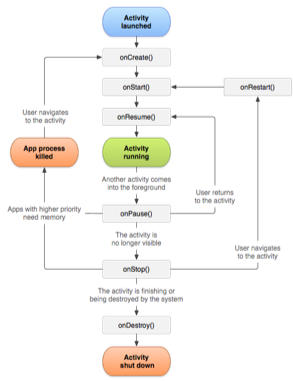
\includegraphics{./figures/Activity_Diagram.png}
    \caption{A flow diagram showing how Android Activities work.}
    \label{fig:my_label}
\end{figure} 

\subsection{Broadcast Receivers}

To understand Broadcast Receivers, we must first look into Android Broadcasts, which are messages that are sent from the Android system and other Android apps whenever an event of interest occurs. These relate to the publish-subscribe design pattern (11) (a messaging pattern that categorises messages into classes when they get published instead of sending these messages directly to specific receivers (12)). Apps can register to receive particular broadcasts so that system changes can be detected in real time. \\*

In order to respond to broadcast messages from the system within our app, we need Broadcast Receivers. Broadcast Receivers are, essentially, “mailboxes” for broadcast messages (9), so whenever Broadcasts relating to a particular system event are sent to some implicit destination, Broadcast Receivers for that event will subscribe to that destination. One very useful property of Broadcast Receivers is that they continue to receive Broadcasts even when the app they have been registered in is not running. Broadcast Receivers are implemented by extending the BroadcastReceiver class. \\*

For a complete list of Android system broadcast actions (as of API 28), please see Figures 2.2 and 2.3 on the following two pages.

\subsection{Handlers}

A Handler is an Android component which allows communication between a background thread and the main UI thread (14). A Handler takes a Java Runnable object, and allows the same task to be scheduled or repeated at a given time interval. Handlers are particularly useful when there are no inbuilt Broadcast Receivers to listen for the variables we want to track, as they can poll the main UI thread at regular time intervals to check whether a variable is changing. The concurrent nature of Handlers makes them ideal for background processing, since potentially slow running operations in the Android app can be performed asynchronously; this improves the overall user experience.

\subsection{Listeners}
An Event Listener is an interface in the Android View class that is used to listen for changes the user had invoked in the UI (for example, an onClickListener could be used to detect whenever the user clicks on a specific button) (16). Listeners contain a single call-back method, and the methods of a Listener are called when the user interacts with the View object that this particular Listener is registered to (where View is the Android class that represents the building block for UI components and is responsible for event handling (17)).

\begin{figure}
    \centering
    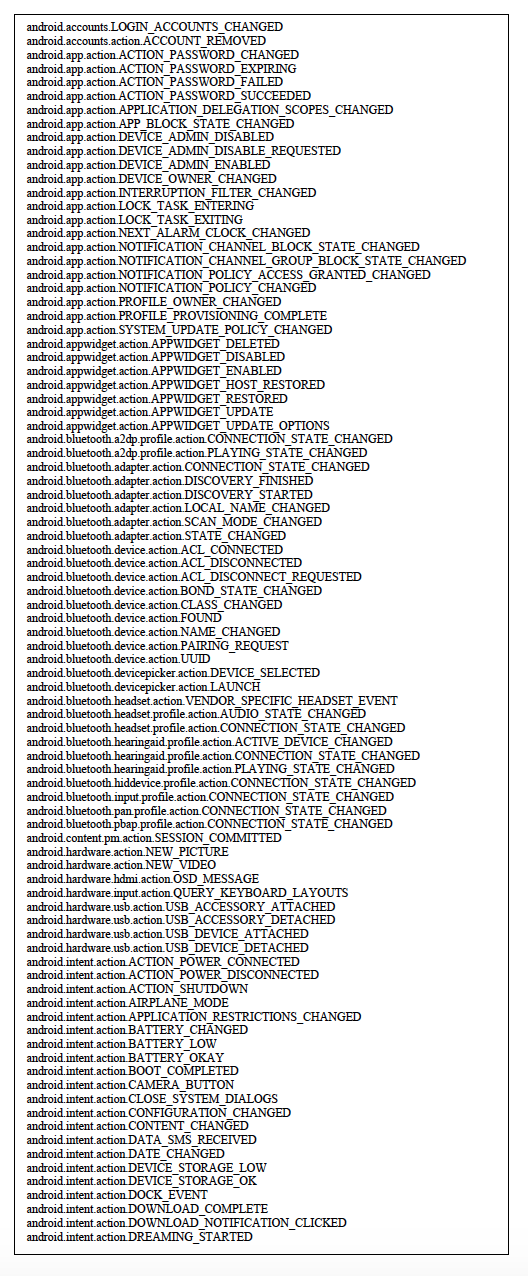
\includegraphics{figures/Broadcast1.png}
    \caption{List of Android Broadcasts (i)}
    \label{fig:my_label}
\end{figure} 

\begin{figure}
    \centering
    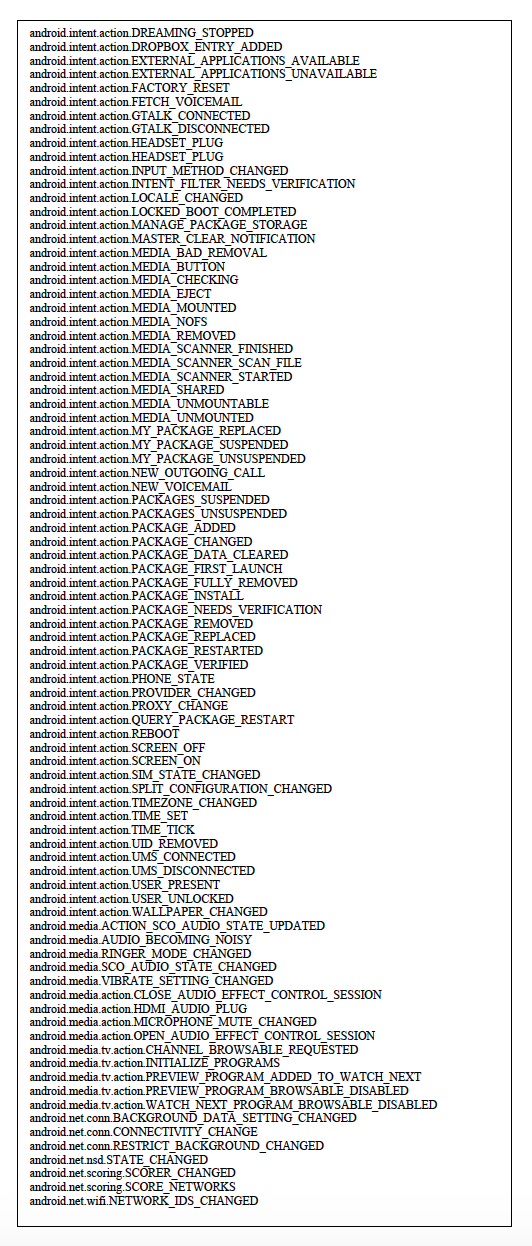
\includegraphics{figures/Broadcast2.png}
    \caption{List of Android Broadcasts (ii)}
    \label{fig:my_label}
\end{figure} 

\newpage
\section{Interaction between components}
\begin{figure}[H]
    \centering
    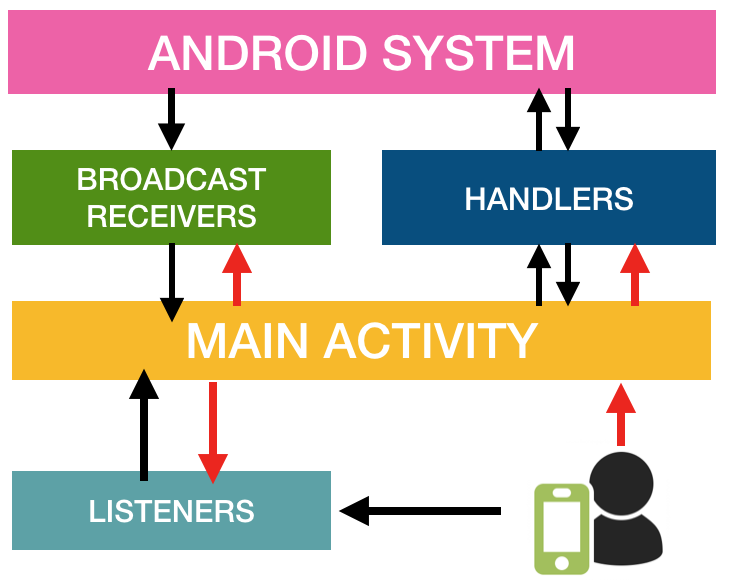
\includegraphics{figures/System_Diagram.png}
    \caption{System diagram showing Android components interacting with each other}
    \label{fig:my_label}
\end{figure}

The system diagram above shows how all of the aforementioned Android components interact with each other in the app.\\*

\textbf{Broadcast Receivers} listen for messages from the Android system to inform them of any changes to the variable being tracked, and also send messages to the Main Activity, specifying which tracking behaviours have changed so that this information can be recorded.\\*

\textbf{Handlers} communicate with the Main Activity in a slightly more complicated way than Broadcast Receivers. Although Handlers do not receive messages from the Android system automatically like Broadcast Receivers, the Main Activity can save the last known state of the variable being tracked and then pass it into the Handler (which takes a Java Runnable object and creates a new thread). The Handler can check whether this variable has changed by polling the Android system at regular time intervals and comparing the new value with the stored one. If anything has changed, the Handler simply sends a message back to the Main Activity so that this information can be recorded. \\*

\textbf{Listeners} rely on user input, and in this app, they relay information back to Main Activity, just like Broadcast Receivers and Handlers.

The \textbf{Main Activity} takes input from the user on what behaviours they want the app to track, and then starts the relevant Broadcast Receivers, Handlers and Listeners needed to track these particular behaviours. The red arrows in the system diagram indicate indirect communication from the user to Broadcast Receivers, Handlers and Listeners, since the user needs to go “through” the Main Activity to start these tracking mechanisms.


\section{Permissions}
The Android security architecture has been designed in a way such that no app, by default, is allowed to perform operations that would have a negative effect on other apps, the operating system, or the user (18). Android permissions were made to support this design - their purpose is to protect the user’s privacy. These permissions can be divided into three broad categories: \textbf{normal} permissions, \textbf{signature} permissions and \textbf{dangerous} permissions. \\*

A \textbf{normal} permission is one which does not pose much risk to the user’s privacy or the device’s operation. If that permission is listed in the Android manifest file, the system automatically grants the permission to the app, and the user is not consulted.\\*

Next, a \textbf{signature} permission is one that the system grants at install time, but only if the app requesting the permission is signed by the same certificate as the app that defines the permission.\\*

Finally, a \textbf{dangerous} permission covers areas that could potentially affect the user’s privacy or the device’s normal operation. In this case, the user must explicitly agree to grant such a permission for the app to be able to provide functionality that depends on the permission.\\*

Lists of each type of permission present in Android (as of API 28) are given below (Figures 2.5, 2.6 and 2.7).

\begin{figure}
    \centering
    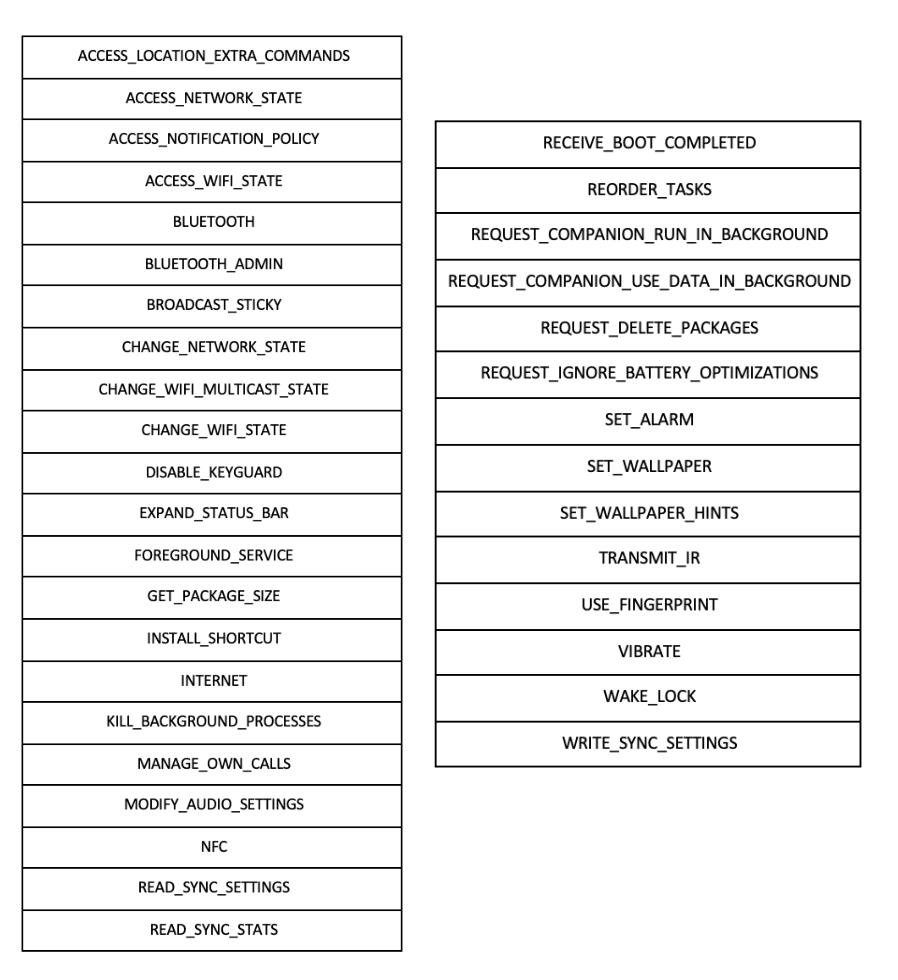
\includegraphics{figures/Normal.png}
    \caption{Normal Permissions}
    \label{fig:my_label}
\end{figure}

\begin{figure}
    \centering
    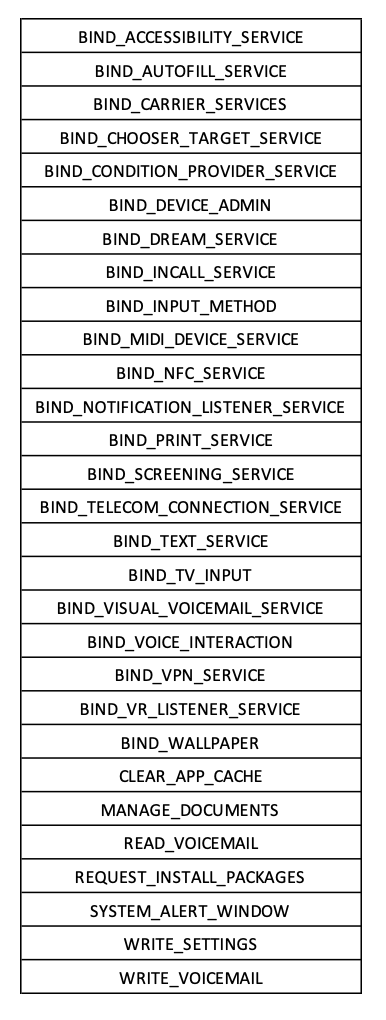
\includegraphics{figures/Signature_Permissions.png}
    \caption{Signature Permissions}
    \label{fig:my_label}
\end{figure}

\begin{figure}
    \centering
    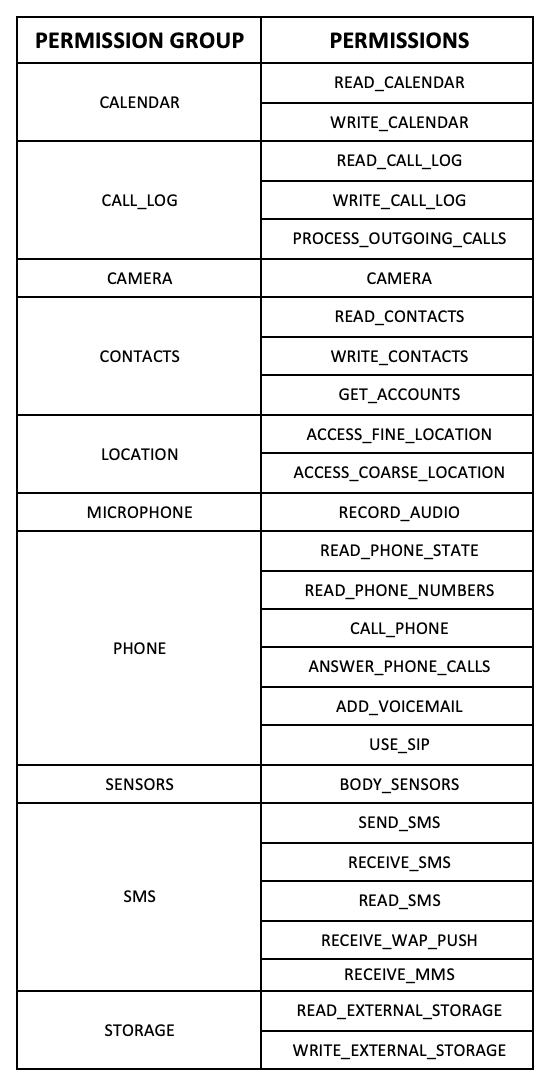
\includegraphics{figures/Dangerous_Permissions.png}
    \caption{Dangerous Permissions}
    \label{fig:my_label}
\end{figure}

%%%%%%%%%%%%%%%%%%%%%%%%%%%%%%%%%%%%
\chapter{Design Overview}

I was given a set of milestones to complete for my app. All of the milestones involved tracking smartphone security behaviours. These security behaviours were divided into two groups: \textbf{technical} configuration actions and \textbf{social} configuration actions.\\*

The \textbf{technical} configuration milestones were as follows:

\begin{enumerate}[label=1.\arabic*]
  \item Track changes in the configuration of Advertising ID
  \item Track changes in the configuration of hide device in Bluetooth settings
  \item Track changes of passcode/PIN for the smartphones screen lock
  \item Detect if the user physically/manually covers her smartphone’s screen when in public spaces
  \item Detect if the user uses adblocker(s)
  \item Detect if the user uses anti-virus app(s)
  \item Detect if the user uses VPN app(s) when connected to a public network
  \item Detect if the user turns off WiFi when not actively being used
\end{enumerate}

Meanwhile, the \textbf{social} configuration milestones were as follows:

\begin{enumerate}[label=2.\arabic*]
    \item Track the source of the app when the user performs financial and/or shopping tasks
    \item Determine when downloading an app, if the user checks (or not) that the app is from the official/expected source (e.g. developer name)
    \item Determine when downloading an app, if the user checks the source of apps (e.g. if they come from Google Play, Amazon App Store or other third party stores)
    \item Determine if the user verifies the recipient/sender before sharing text messages or other information using smartphone apps
    \item Determine if the user deletes any online communications (i.e., texts, emails, social media posts) that look suspicious
    \item Determine if the user pays attention to the pop-ups on her smartphone when connecting it to another device (e.g. laptop, desktop)
\end{enumerate}
%%%%%%%%%%%%%%%%%%%%%%%%%%%%%%%%%%%%
\chapter{Experimental Results}


%%%%%%%%%%%%%%%%%%%%%%%%%%%%%%%%%%%%
\chapter{Conclusion}


%% bibliography
\bibliographystyle{apa}


\end{document}
